\chapter{Digital Twin Implementation}\label{ch:implementation}

The implementation of the \acrshort{dt} is based on the hypothetical home described in Chapter~\ref{ch:hypothetical_home}.

\begin{itemize}
    \item No physical twin exists yet, development of the digital twin is the first step.
    \item What the digital twin does.
          \begin{itemize}
              \item Read routines and appliances;
              \item Show current and future consumption of appliances;
              \item Simulate new routines;
              \item Evaluate conflicts;
              \item Produce errors and recommendations.
          \end{itemize}
    \item Appliance state modeling.
    \item Conflict scenarios.
    \item Implementation details
          \begin{itemize}
              \item Appliance and routine data;
              \item Python libraries;
              \item REST API in FastAPI;
              \item Frontend in React.
          \end{itemize}
\end{itemize}

\section{Configuration}

\begin{lstlisting}[language=json,caption={Example of a configuration file.},label=code:configuration,float,floatplacement=H]
[energy]
max_power = 3
energy_rates_number = 2
energy_rates_prices = [
    0.131870,
    0.111492,
]

[database]
type = "json"
appliances_dir = "json/appliances"
routines_dir = "json/routines"
test_routines_dir = "json/test_routines"
\end{lstlisting}

The \acrshort{dt} can read a configuration file written in TOML, located at the path set by the \texttt{CONFIG\_PATH} environment variable. The configuration file contains the following information:
\begin{itemize}
    \item \texttt{energy}: energy related parameters.
          \begin{itemize}
              \item \texttt{max\_power}: the maximum power draw, in kW;
              \item \texttt{energy\_rates\_number}: the number of energy rates, e.g. 2 means dual-rate;
              \item \texttt{energy\_rates\_prices}: the price for each energy rate, in \texteuro/kWh.
          \end{itemize}
    \item \texttt{database}: database related parameters.
          \begin{itemize}
              \item \texttt{type}: the type of database, only \texttt{json} is supported at the moment;
              \item \texttt{appliances\_dir}: the directory where the appliances JSON files are stored;
              \item \texttt{routines\_dir}: the directory where the routine JSON files are stored;
              \item \texttt{test\_routines\_dir}: the directory where the routine JSON files for tests are stored;
          \end{itemize}
\end{itemize}

The number of energy rates follows the Delibera n.181/06\footnote{\url{https://www.arera.it/atti-e-provvedimenti/dettaglio/06/181-06} (visited on 2024, February 22)} by the \acrfull{arera}, which defines the conditions for the application of multiple-rate tariffs. A maximum of three rates (F1, F2, F3) is allowed, where F1 goes from 8:00 to 19:00, monday to friday, F2 goes from 7:00 to 8:00 and from 19:00 to 23:00, monday to friday, and from 7:00 to 23:00 on saturday, and F3 goes from 23:00 to 7:00, monday to saturday, and from 23:00 to 24:00 on sunday. The allocation of the rates, represented in Figure~\ref{fig:costs_matrix} depends on the time of the day and the day of the week. The actual number of rates can be lower than three, depending on the contract with the energy provider. If only two rates are quoted, the rates F2 and F3 can be grouped to form a dual rate tariff (F1, F23).

\begin{figure}
    \centering
    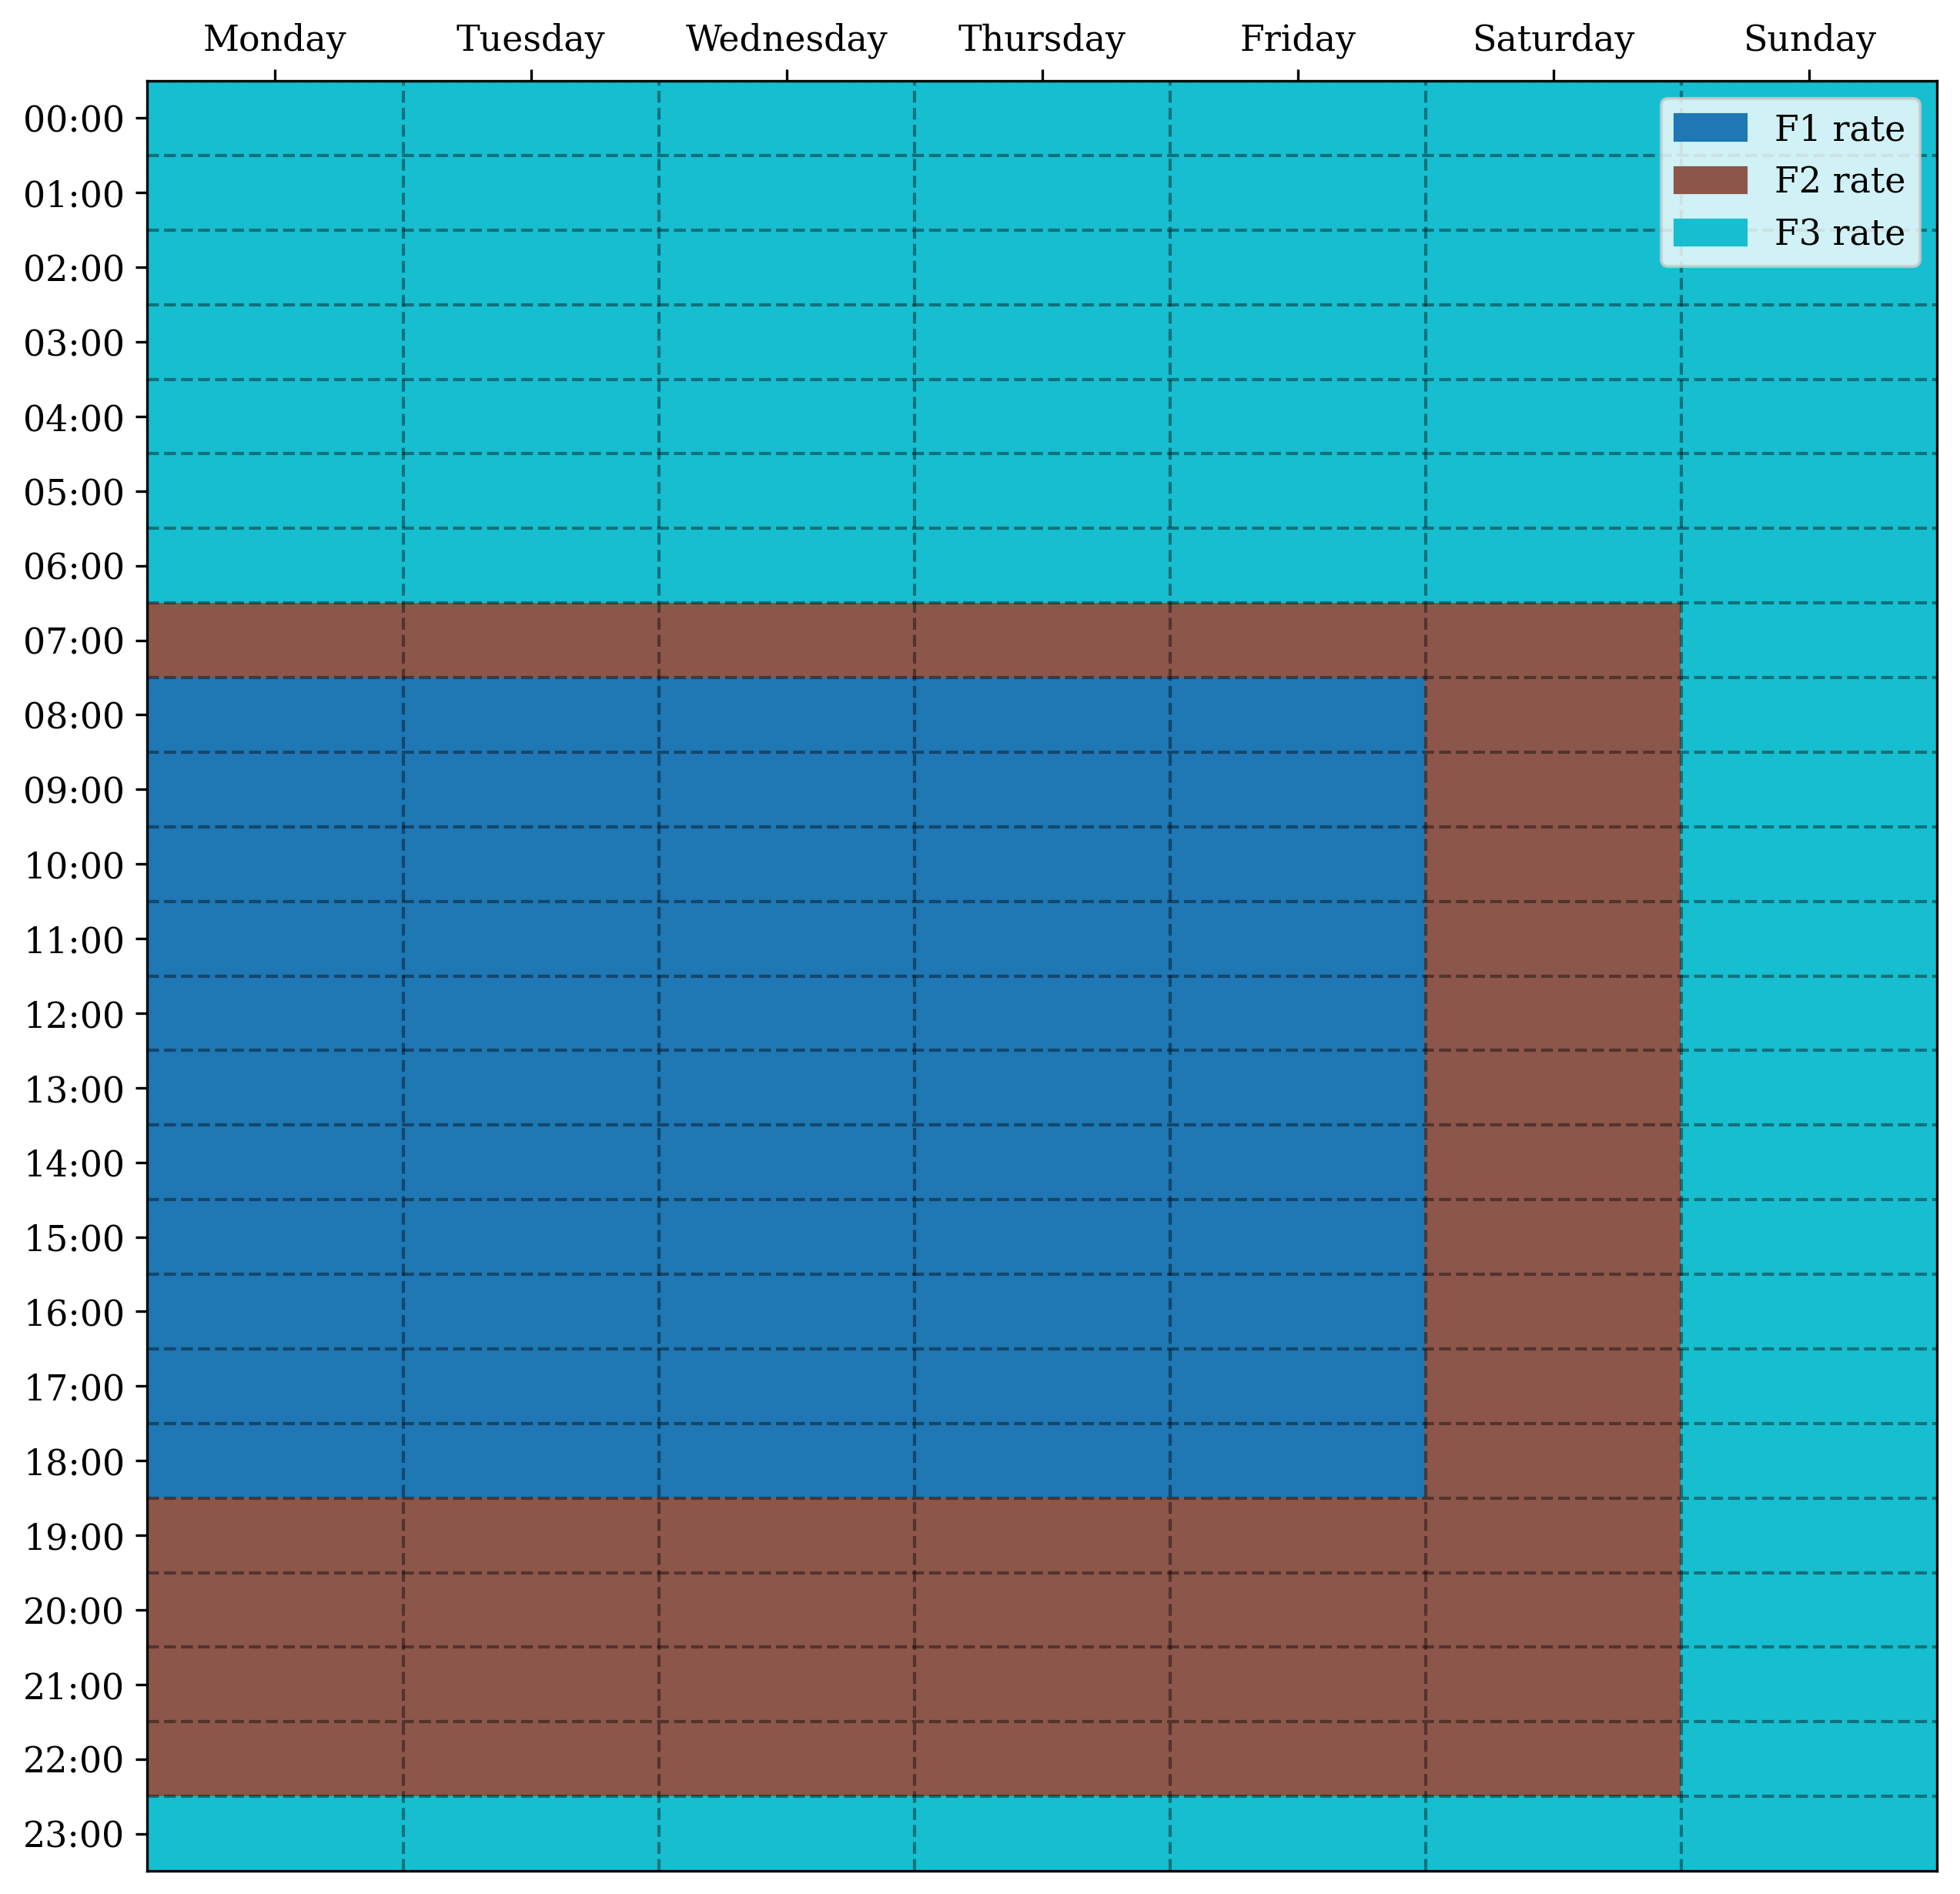
\includegraphics[width=0.9\textwidth]{images/costs.png}
    \caption[Electricity tariffs applied in italy for every day of the week]{Electricity tariffs applied in italy for every day of the week. F1 is the peak rate, F2 is the mid-level, and F3 is off-peak}
    \label{fig:costs_matrix}
\end{figure}

The configuration used for the development of the \acrshort{dt} is shown in Code Sample~\ref{code:config}. Two energy rates are used, where the prices correspond to the \acrfull{pun} values, i.e. the Single National Price values, refferring to the month of December 2023. The \acrshort{pun} is calculated by the \acrfull{gme}\footnote{\url{https://www.mercatoelettrico.org/En/default.aspx} (visited on 2024, February 22)}, as the weighted average of the prices of the energy markets, and is used as a reference for the energy costs in Italy. The maximum power draw is set to $3kW$, which is the standard maximum power supply before cut off in Italy.

\section{Appliance and Routine Data}

The data of the appliances in the hypothetical home and the routines registered by the end users are stored as JSON files.
Examples of appliance JSON files for the dish washer and the washing machine are shown in Code Samples~\ref{code:appliance_dish_washer} and~\ref{code:appliance_washing_machine}, respectively. The files contain the following information:
\begin{itemize}
    \item \textit{ID}: a unique integer number identifying the appliance among other appliances;
    \item \textit{Device}: the type of appliance, e.g. \textit{dish washer}
    \item \textit{Manufacturer} (optional): the manufacturer of the appliance, e.g. \textit{Whirlpool};
    \item \textit{Model} (optional): the model of the appliance e.g. \textit{ADF 555 IX};
    \item \textit{Location}: the room where the appliance is located, e.g. \textit{kitchen};
    \item \textit{Modes}: the list of operation modes available for the appliance. Every appliance has at least an \textit{off} mode, that consumes no power. For each mode the following information is provided:
          \begin{itemize}
              \item \textit{ID}: a unique integer number identifying the mode among the other modes of the appliance;
              \item \textit{Name}: the name of the mode, e.g. \textit{intensive};
              \item \textit{Power consumption}: the mean power consumption of the appliance in the mode, in Watts;
              \item \textit{Default duration} (optional): the default duration of the operation mode, which will be used if the user does not specify a duration in the routine.
          \end{itemize}
\end{itemize}

\begin{lstlisting}[language=numbered,caption={JSON file describing the dish washer},label=code:appliance_dish_washer,float,floatplacement=H]
{
  "id": 3,
  "device": "dish washer",
  "manufacturer": "Whirlpool",
  "model": "ADG 555 IX",
  "location": "kitchen",
  "modes": [
    {
      "id": 0,
      "name": "off",
      "power_consumption": 0
    },
    {
      "id": 1,
      "name": "daily",
      "power_consumption": 810,
      "default_duration": 10260
    },
    ...	
    {
      "id": 6,
      "name": "pre-wash",
      "power_consumption": 10,
      "default_duration": 660
    }
  ]
}
\end{lstlisting}

\begin{lstlisting}[language=numbered,caption={[JSON file describing the washing machine]JSON file describing the washing machine.},label=code:appliance_washing_machine,float,floatplacement=H]
{
	"id": 15,
	"device": "washing machine",
	"manufacturer": "Zanussi",
	"model": "F1215",
	"location": "bathroom",
	"modes": [
		{
			"id": 0,
			"name": "off",
			"power_consumption": 0
		},
		{
			"id": 1,
			"name": "cotton 90",
			"power_consumption": 2000,
			"default_duration": 8700
		},
		...	
		{
			"id": 7,
			"name": "wool",
			"power_consumption": 450,
			"default_duration": 3300
		}
	]
}
\end{lstlisting}

An example of a routine which starts the dish washer in \textit{intensive} mode and the washing machine in \textit{cotton 90} mode at 14:00 is shown in Code Sample~\ref{code:routine_wash_everything}. The file contains the following information:
\begin{itemize}
    \item \textit{ID}: a unique integer number identifying the routine among other routines;
    \item \textit{Name}: a name for the routine, e.g. \textit{wash everything};
    \item \textit{When}: the time when the routine is executed, in the format \textit{HH:MM};
    \item \textit{Actions}: the list of actions that the routine involves. For each action the following information is provided:
          \begin{itemize}
              \item \textit{ID}: a unique integer number identifying the action among the other actions of the routine;
              \item \textit{Appliance ID}: the ID of the appliance involved in the action;
              \item \textit{Duration} (optional): the duration of the operation mode, in minutes. If not specified, the default duration of the mode is used.
          \end{itemize}
\end{itemize}

\begin{lstlisting}[language=numbered,caption={[Example of a routine with two actions]Example of a routine with two actions.},label=code:routine_wash_everything,float,floatplacement=H]
{
    "id": 5,
    "name": "Wash everything",
    "when": "14:00",
    "enabled": true,
    "actions": [
        {
            "id": 0,
            "appliance_id": 15,
            "mode_id": 1
        },
        {
            "id": 1,
            "appliance_id": 3,
            "mode_id": 1
        }
    ]
}
\end{lstlisting}

\section{Appliance State Modeling}

Using the defined routines, the \acrshort{dt} is capable of creating a \textit{state map} of the appliances throughout the day, which tracks the operation mode in which each appliance is set for each minute of the day. The state map is used to evaluate the conflict scenarios and to simulate the addition of a new routine. An example of a state map is shown in Figure~\ref{fig:state_map}, which shows the operation modes of the appliances in the hypothetical home throughout the day, using a predefined set of routines.

\begin{figure}
    \centering
    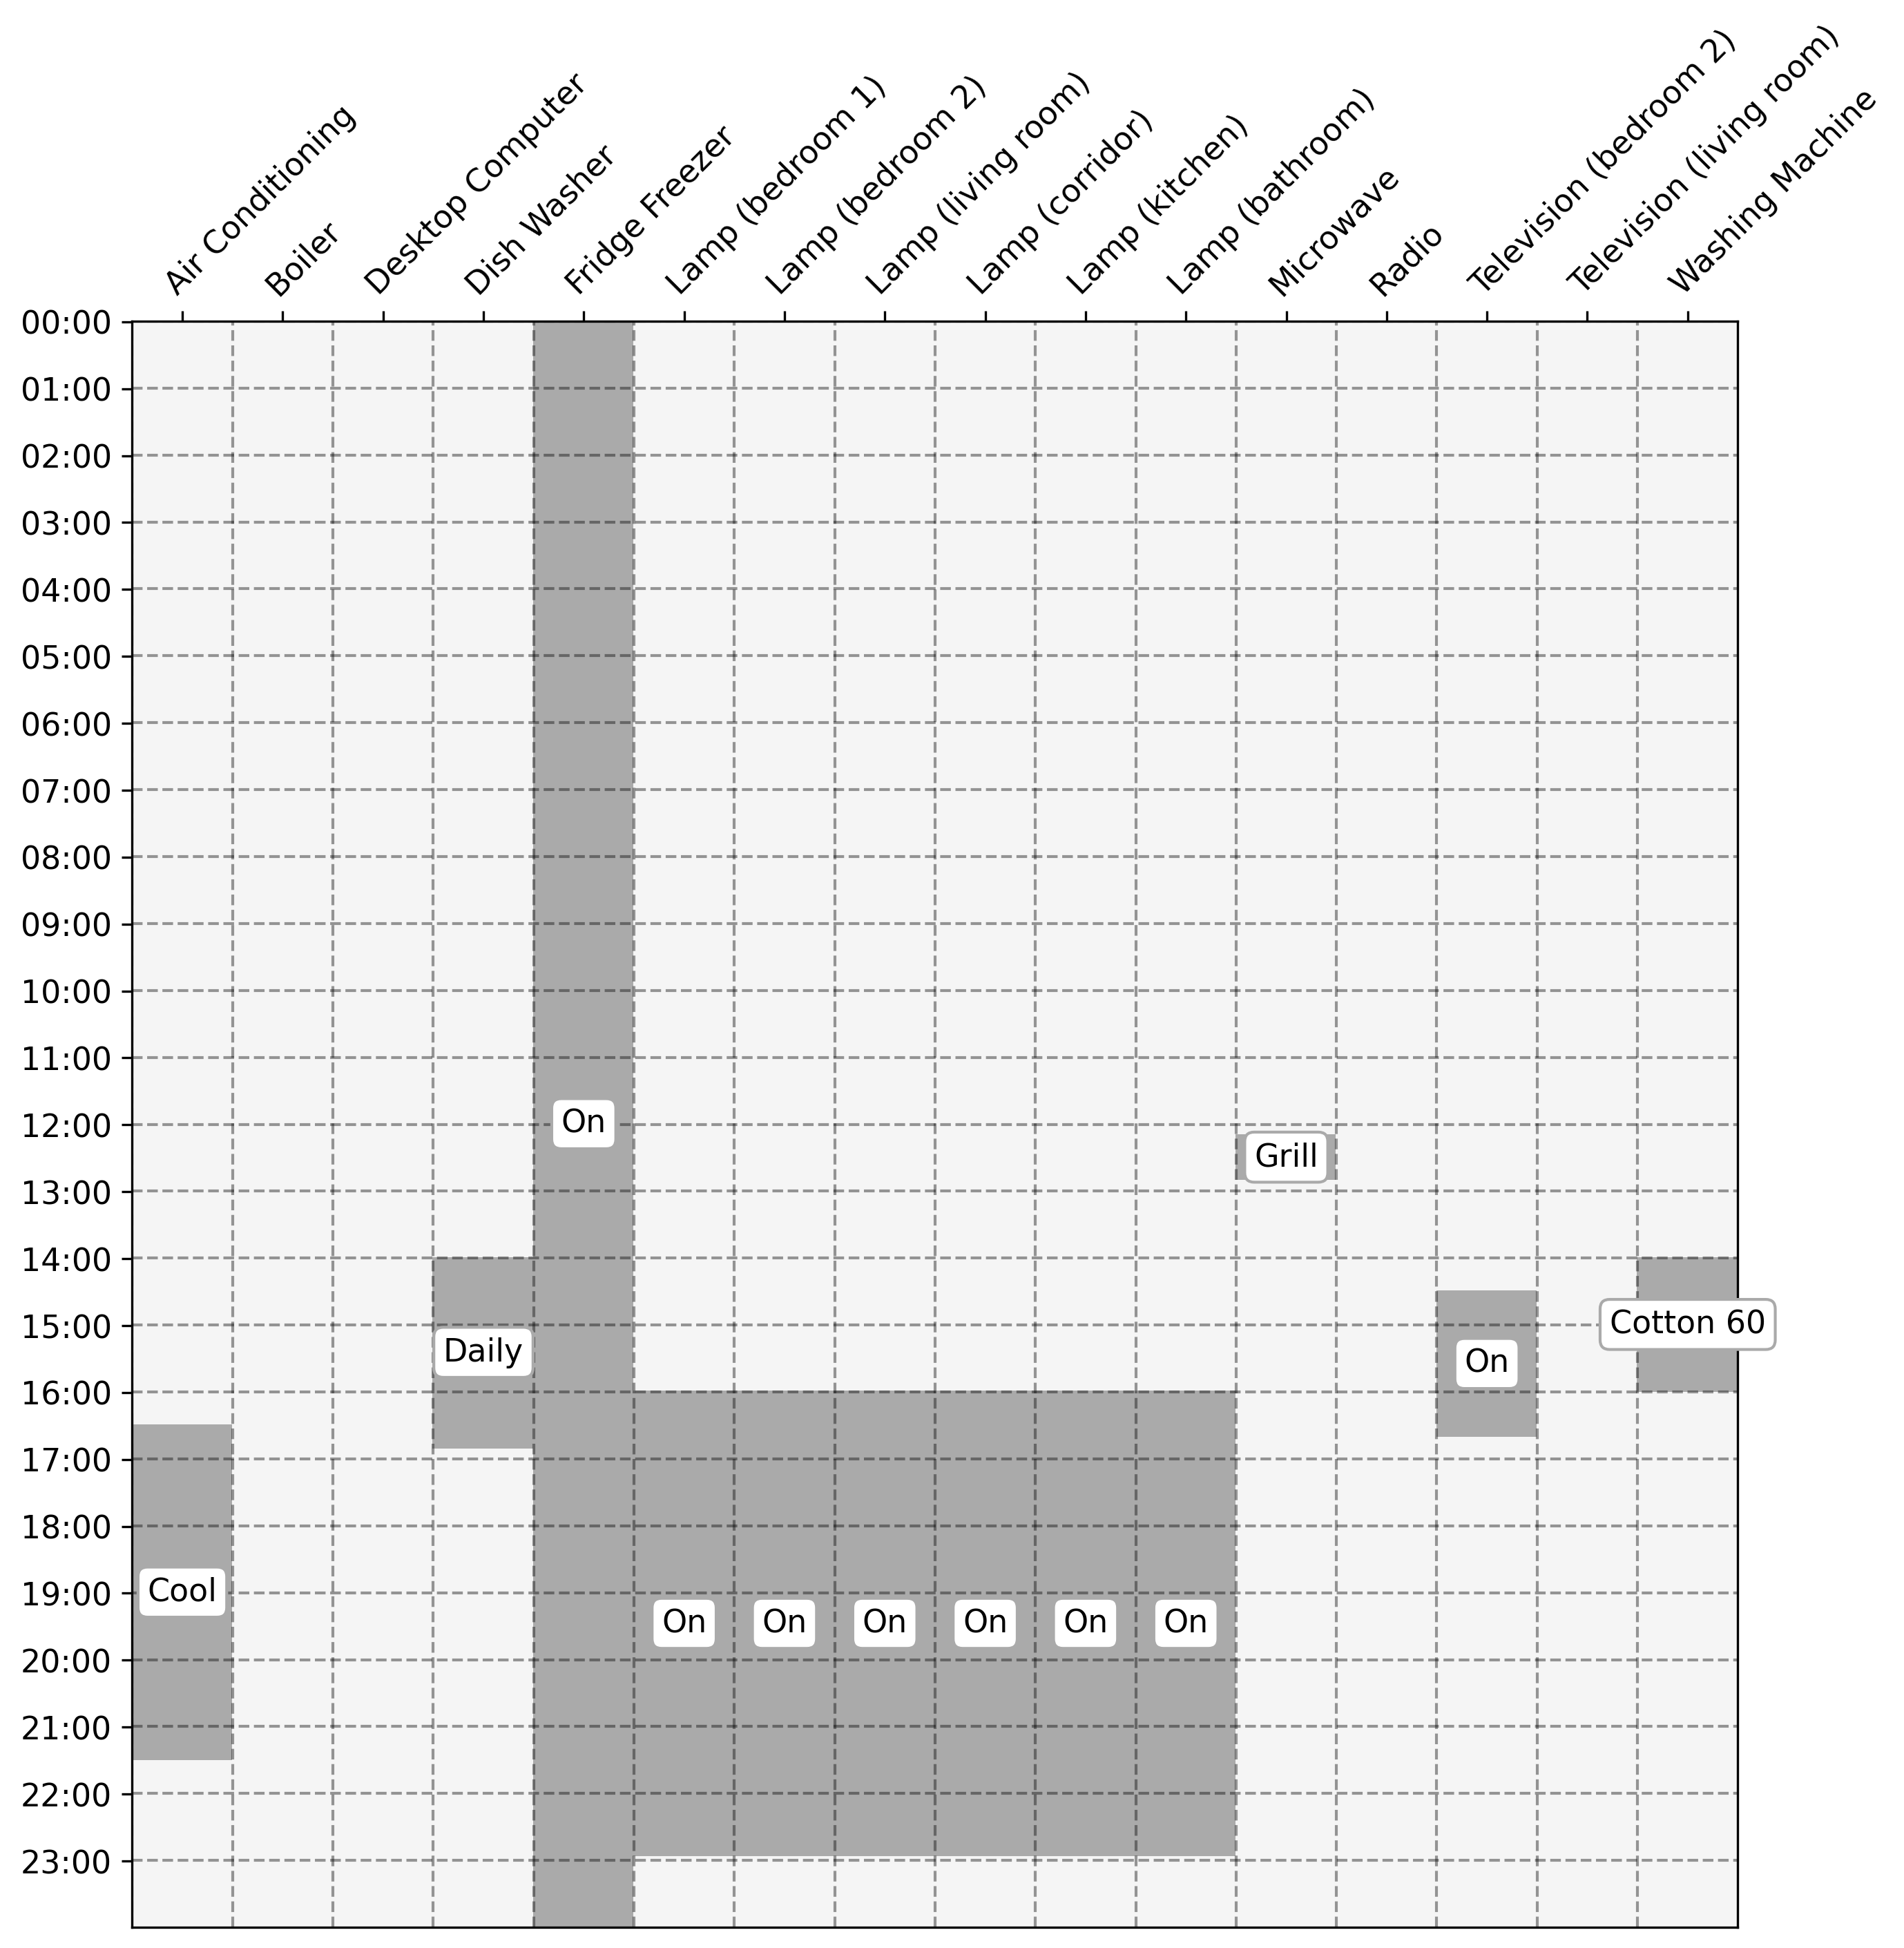
\includegraphics[width=0.9\textwidth]{images/real_matrix.png}
    \caption[Example of a state map.]{Example of a state map. The matrix shows the operation modes of the appliances in the hypothetical home throughout the day, using a predefined set of routines.}
    \label{fig:state_map}
\end{figure}

The matrix is implemented using the \texttt{ndarray} class provided by the NumPy library~\parencite{harrisArrayProgrammingNumPy2020}, which is a n-dimensional array of integers. As described in the Numpy N-Dimensional Array Reference\footnote{\url{https://numpy.org/doc/1.26/reference/arrays.ndarray.html}}, an instance of the \texttt{ndarray} class consists of a contiguous monodimensional memory segment, which combined with an indexing scheme allows to represent multidimensional arrays, mapping integers to the various elements that compose the memory block.

Each row of the matrix corresponds a minute of the day, and each column represents an appliance, by associating the appliance ID to the column index. For example, the first column of the matrix (index $0$) corresponds to the appliance with index 0. The value of each cell is the ID of the operation mode in which the appliance is set at that minute. Given that in a day there are $24 \times 60 = 1440$ minutes, and the hypothetical home has 15 appliances, the state map is a $1440 \times 15$ matrix. The type of the matrix is \textit{uint8}, which allows to store integers from 0 to 255, which is enough to store the IDs of the operation modes of the appliances. The total memory used by the state map is $1440 \times 15 \times 8 = 172800$ bits, which corresponds to roughly $21$ kilobytes.

\section{Simulation of New Routines}

\begin{figure}
    \centering
    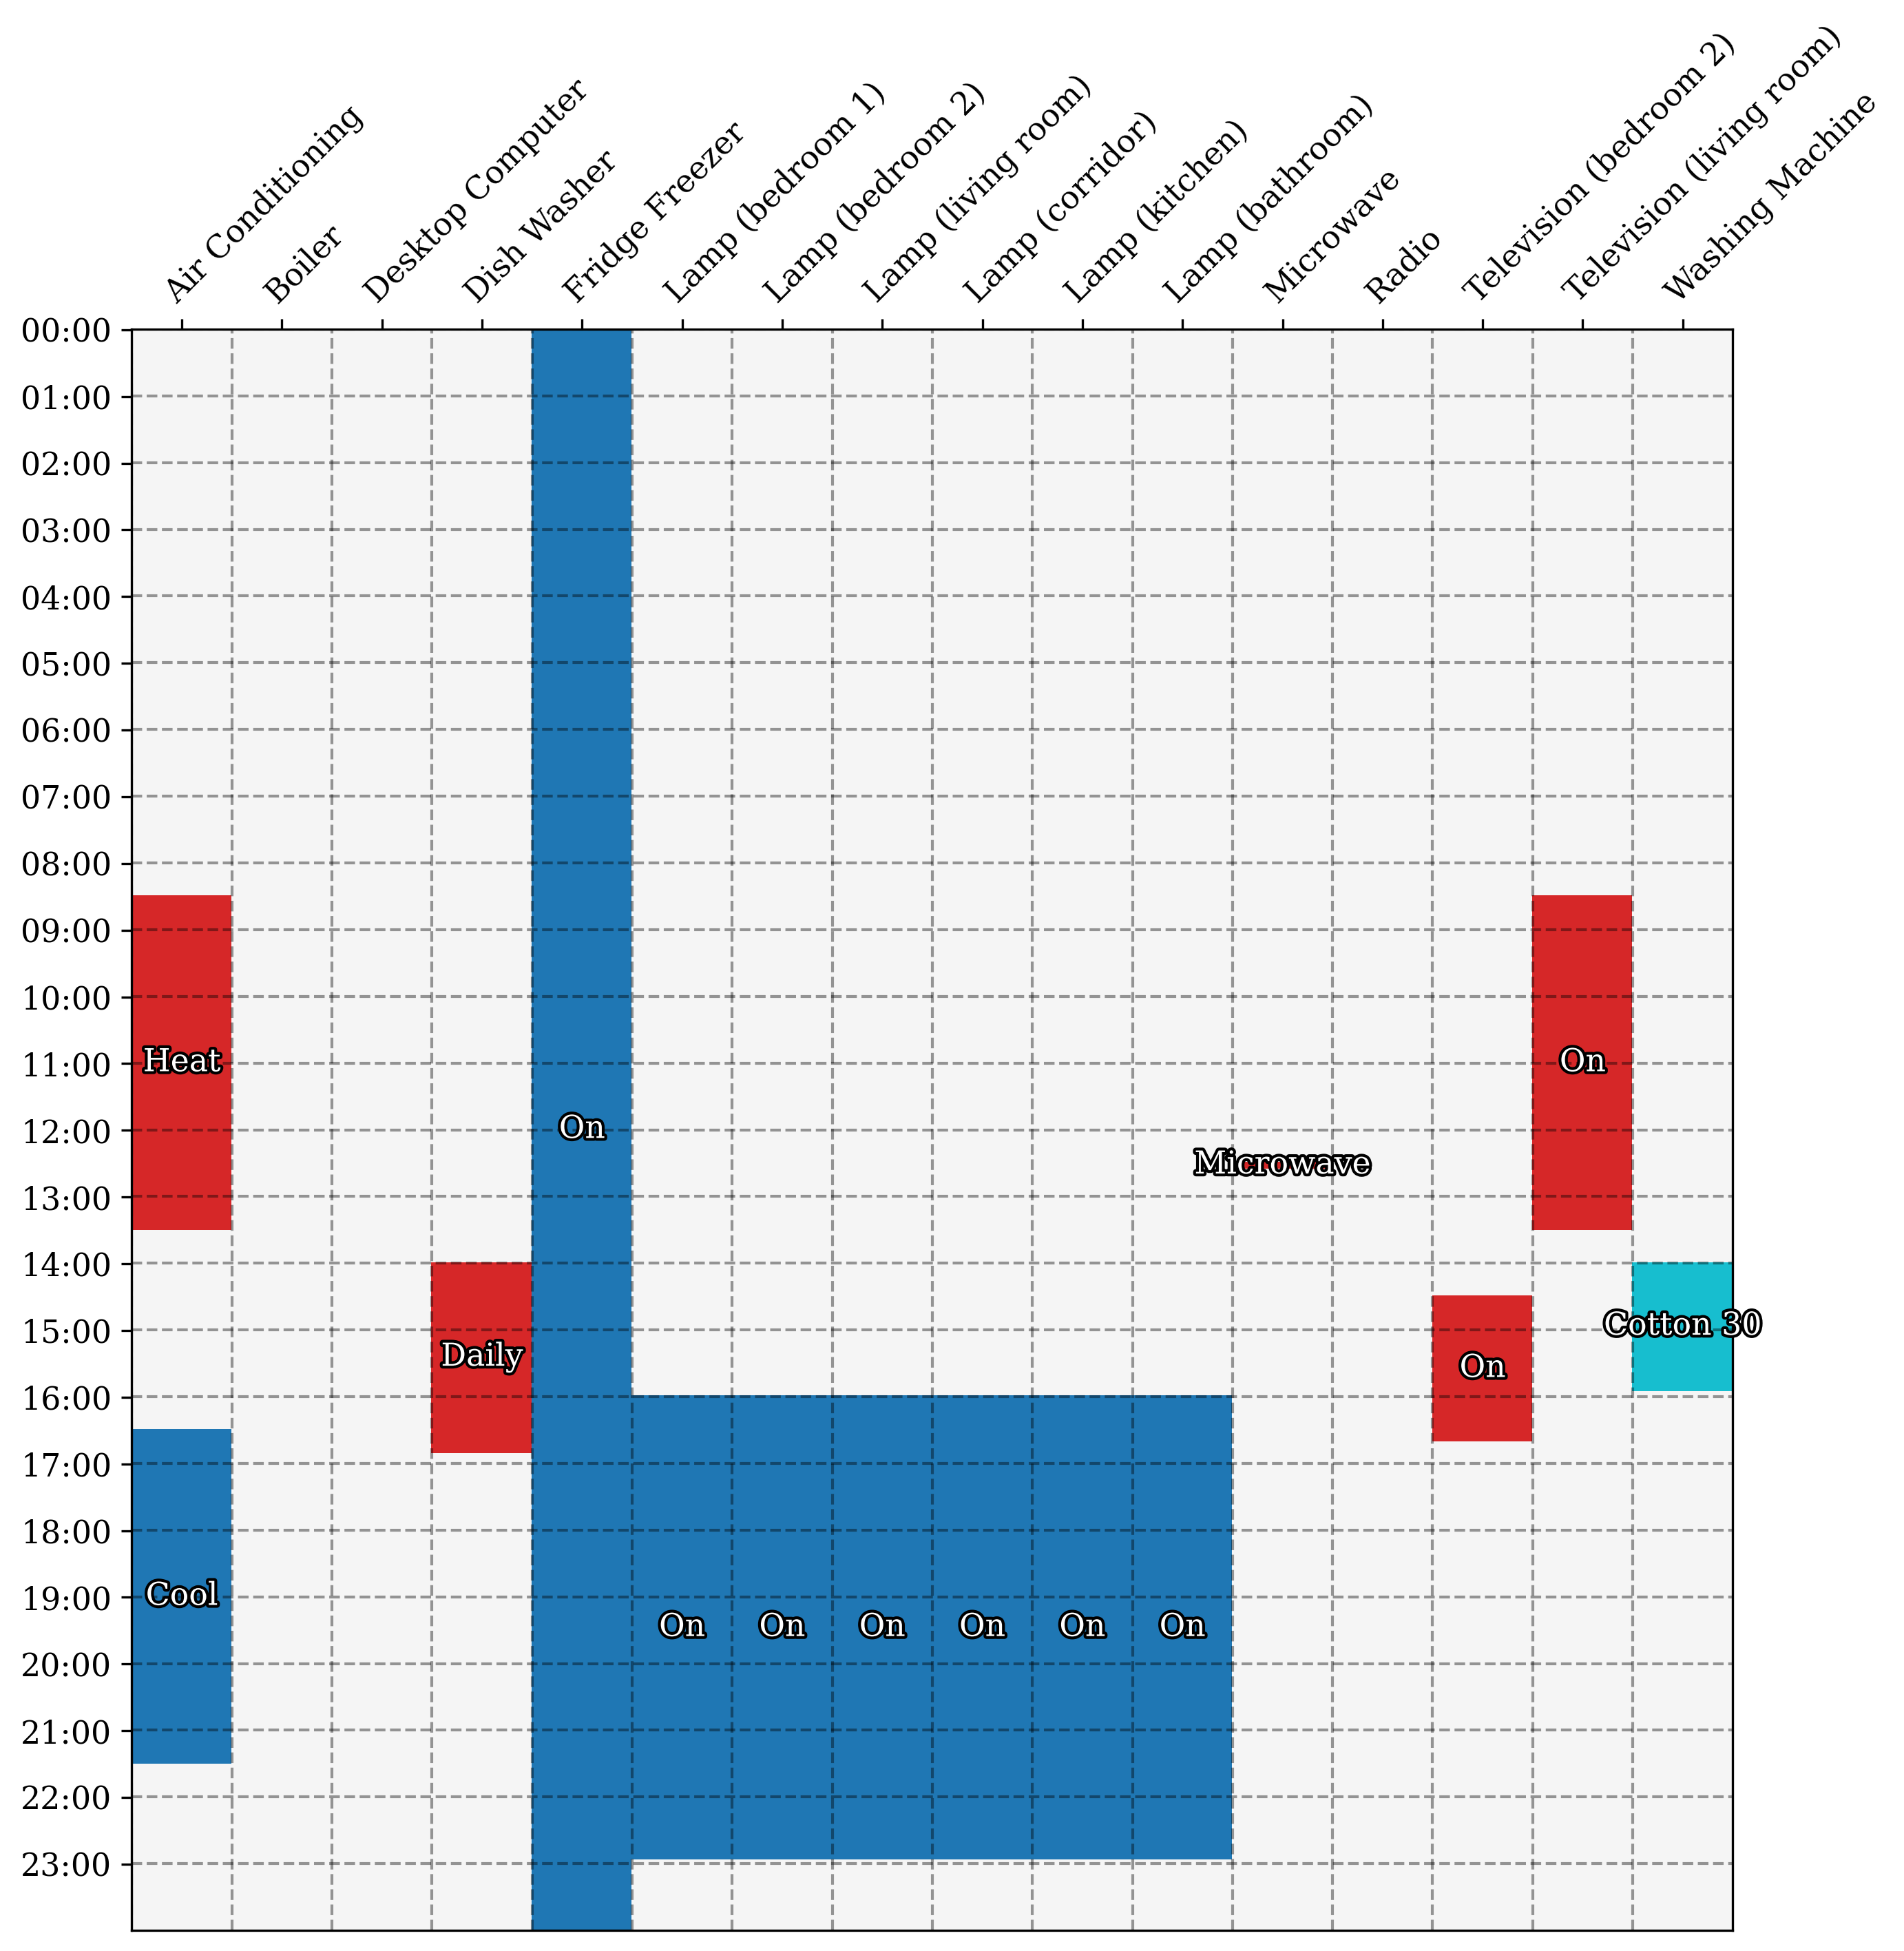
\includegraphics[width=0.9\textwidth]{images/simulated_matrix.png}
    \caption{Simulated matrix.}
    \label{fig:simulated_consumption_matrix}
\end{figure}

When simulating the addition of a new routine, it is possible that it causes a conflict with the existing routines. The \acrshort{dt} is capable of evaluating such conflicts and shows proper messages to the user. It is assumed that the existing routines are already consistent and conflict-free.

The \acrshort{dt} evaluates the potential conflicts and produces \textit{errors} or \textit{recommendations}, or both. An error occurs when a conflict creates an inconsistency among the routines, e.g. when two routines include actions that contradict each other, or that put the power draw over a maximum limit. Errors halt the simulation and prevent further evaluation. Recommendations are either warnings about minor conflicts that do not affect the consistency, or suggestions to improve the user experience or save energy. A recommendation does not interrupt the simulation and allows for further evaluation. This means that the digital twin can provide multiple recommendations for different conflicts, but at most one error is returned at a time.

The expected conflict scenario are the following:
\begin{enumerate}[label={\textit{S\arabic*.}}, leftmargin=3.5em]
    \item \textit{An appliance has conflicting operation modes in the same time interval}. This occurs when a simulated routine assigns an appliance a different operation mode than the one assigned by the existing routines in the same time interval. If the simulated routine assigns the same operation mode as the existing routines, there is no conflict. For instance, the AC is set to \textit{heat} from 8:00 to 12:00. A simulated routine that sets the AC to \textit{cold} from 10:00 to 11:00 causes a conflict. The digital twin rejects the simulated routine with an error that specifies the conflicting action and the existing routine and action. It also suggests deactivating the existing routine instead. This may be useful, for example, in weather conditions with sudden temperature changes, where the user may want to adjust the AC temporarily. If the simulated routine does not cause an inconsistency, e.g. it sets the AC to \textit{heat} from 11:00 to 13:00, then the digital twin accepts the simulated routine with a recommendation to modify the existing routine action to set \textit{heat} from 8:00 to 13:00.

    \item \textit{The power consumption exceeds a maximum limit at any time}. The digital twin rejects any routine that causes the power consumption to go beyond the maximum limit at any point. This limit could be the maximum power supply before cut off, e.g. $3kW$ in Italy. For example, if the microwave is in \textit{microwave mode}, the dishwasher is in \textit{intensive} mode, and the simulated routine sets the washing machine to \textit{cotton 60} mode at 14:00, the digital twin produces an error and advises a better start time for the washing machine.

    \item \textit{A better start time can be determined}. The digital twin tries to find a more economical start time for each action of the simulated routine, using pre-set electricity costs. This is important, for example, if the user has a variable electricity tariff, where it is less expensive to run appliances at night. If the electricity cost is constant throughout the day, this step can be ignored. The digital twin evaluates each action of the simulated routing sequentially, taking into account the best start time of the previous actions. For instance, if the best start time of action 1 of the simulated routine is 15:30, the digital twin should use that as a reference when evaluating action 2.

    \item \textit{An appliance is activated manually by the end user}. This scenario requires the digital twin to monitor the running state of appliances, in addition to the routines. Before executing any routine actions, the digital twin should check for conflicts with scenarios S1 and S2, using the current state of the appliances as well. If the scenarios produce an error, the conflicting actions should be prevented from running. Actions that are conflict-free can still be executed. Any recommendation produced can be displayed to the user to alert them and offer alternatives on what to do.
\end{enumerate}
The implementation of the digital twin developed for this thesis only covers conflicts S1-S4, while conflict S5 is left as a future development.

\section{REST API}

\begin{table}
    \centering
    \resizebox{\textwidth}{!}{%
        \begin{tblr}{ll>{\raggedright}p{.18\textwidth}p{.18\textwidth}lp{.5\textwidth}}
            \hline
            Endpoint                    & Method & Path parameters             & Query Parameters        & Body parameters     & Description                                                                                                                         \\ \hline
            /consumption                & GET    & date and time               &                         &                     & Returns a list of energy consumption values of all appliances at the given date and time.                                           \\
            /consumption                & GET    & appliance id, date and time &                         &                     & Returns the energy consumption value of the given appliance at the given date and time.                                             \\
            /consumption/total          & GET    &                             & list of dates and times &                     & Returns the list of total energy consumption of all appliances at the given dates and times.                                        \\
            /consumption/total          & GET    & date and time               &                         &                     & Returns the total energy consumption of all appliances at the given date and time.                                                  \\ \hline[dashed]
            /appliance                  & GET    &                             &                         &                     & Returns the list of all appliances                                                                                                  \\
            /appliance                  & GET    & appliance id                &                         &                     & Returns a specific appliance                                                                                                        \\ \hline[dashed]
            /routine                    & GET    &                             &                         &                     & Returns the list of all routines                                                                                                    \\
            /routine                    & GET    & routine id                  &                         &                     & Returns a specific routine                                                                                                          \\ \hline[dashed]
            /simulate                   & POST   &                             &                         & routine to simulate & Simulates the addition of a routine and returns a list of recommendations and errors (if any)                                       \\
            /simulate/consumption       & POST   & date and time               &                         & routine to simulate & Simulates the addition of a routine and returns a list of energy consumption values of all appliances at the given date and time    \\
            /simulate/consumption       & POST   & appliance id, date and time &                         & routine to simulate & Simulates the addition of a routine and returns the energy consumption value of the given appliance at the given date and time      \\
            /simulate/consumption/total & POST   & date and time               &                         & routine to simulate & Simulates the addition of a routine and returns the list of total energy consumption of all appliances at the given dates and times \\
            /simulate/consumption/total & POST   &                             & list of dates and times & routine to simulate & Simulates the addition of a routine and returns the total energy consumption of all appliances at the given date and time           \\ \hline
        \end{tblr}%
    }
    \caption{Endpoints of the \acrshort{dt}'s REST API.}
    \label{tab:rest_api_endpoints}
\end{table}

\section{Frontend}

\begin{figure}
    \centering
    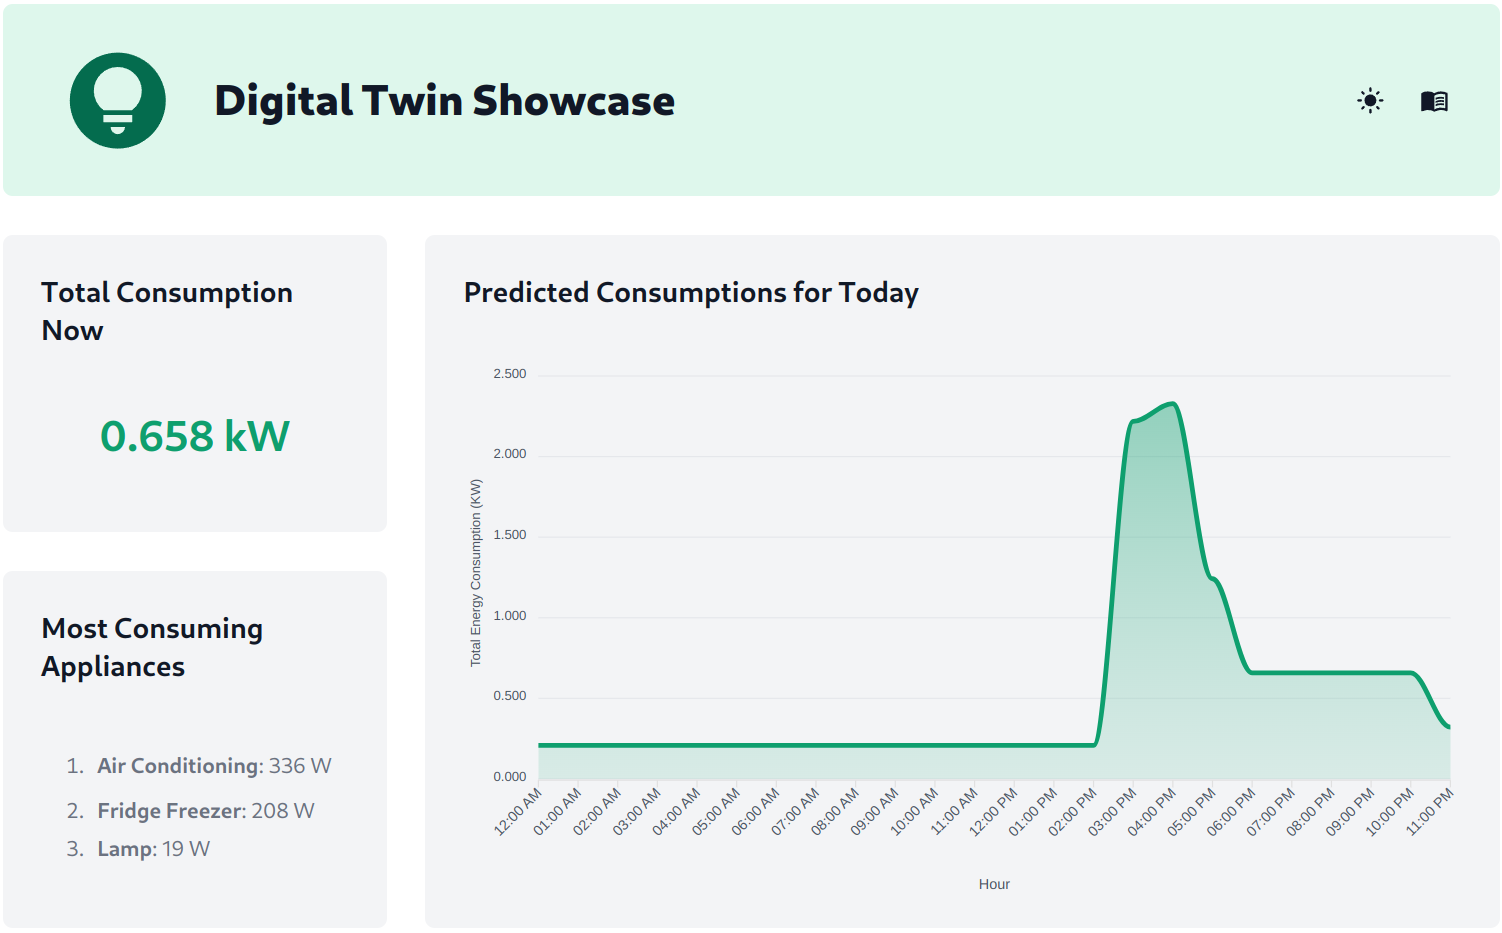
\includegraphics[width=0.9\textwidth]{images/frontend/header.png}
    \caption{Showcase Frontend Application}
    \label{fig:frontend_header}
\end{figure}

\begin{figure}
    \centering
    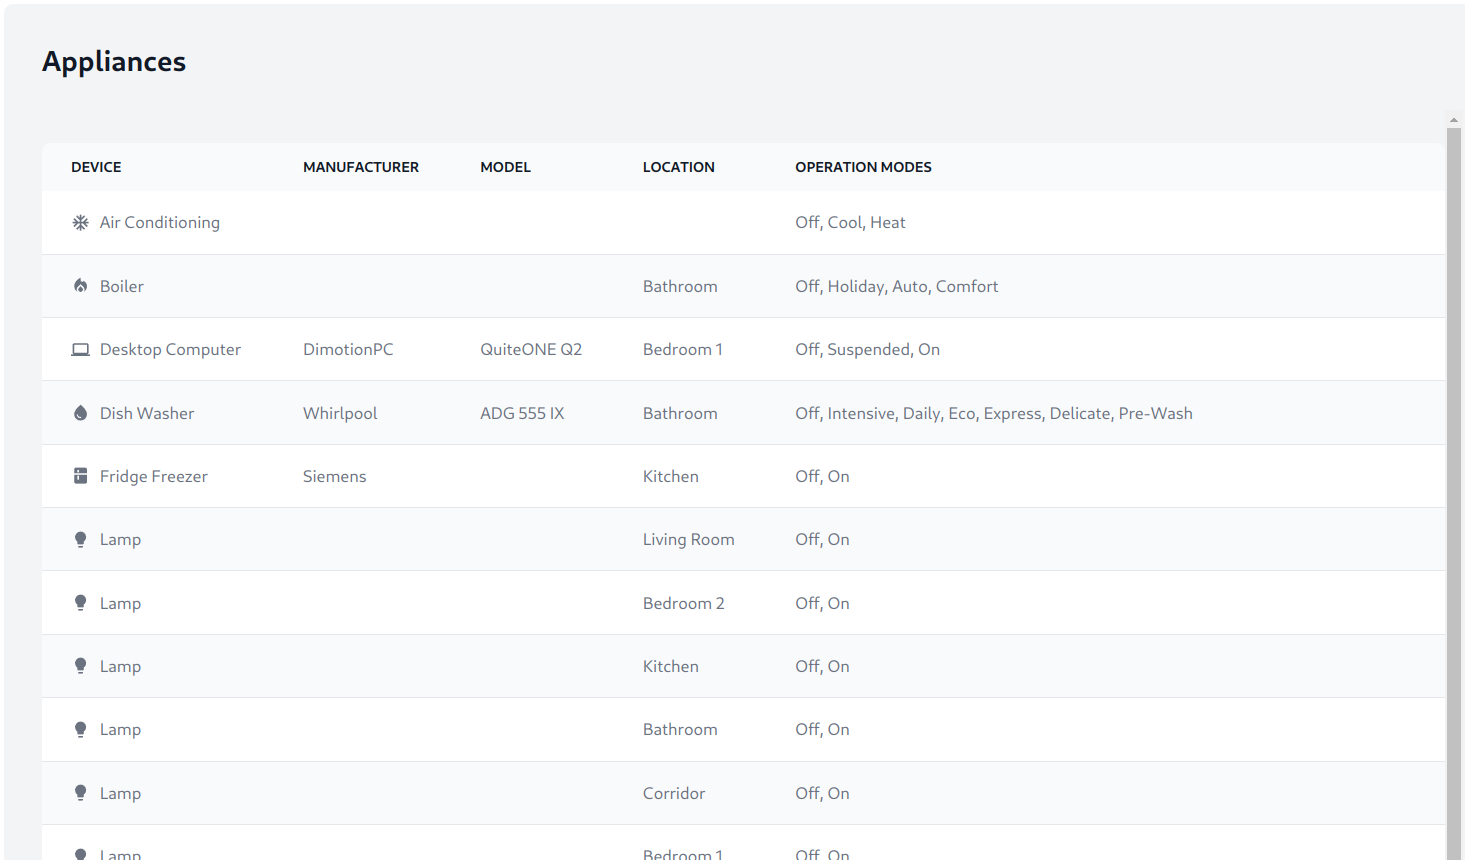
\includegraphics[width=0.9\textwidth]{images/frontend/appliances.png}
    \caption{Showcase Frontend Application}
    \label{fig:frontend_appliances}
\end{figure}

\begin{figure}
    \centering
    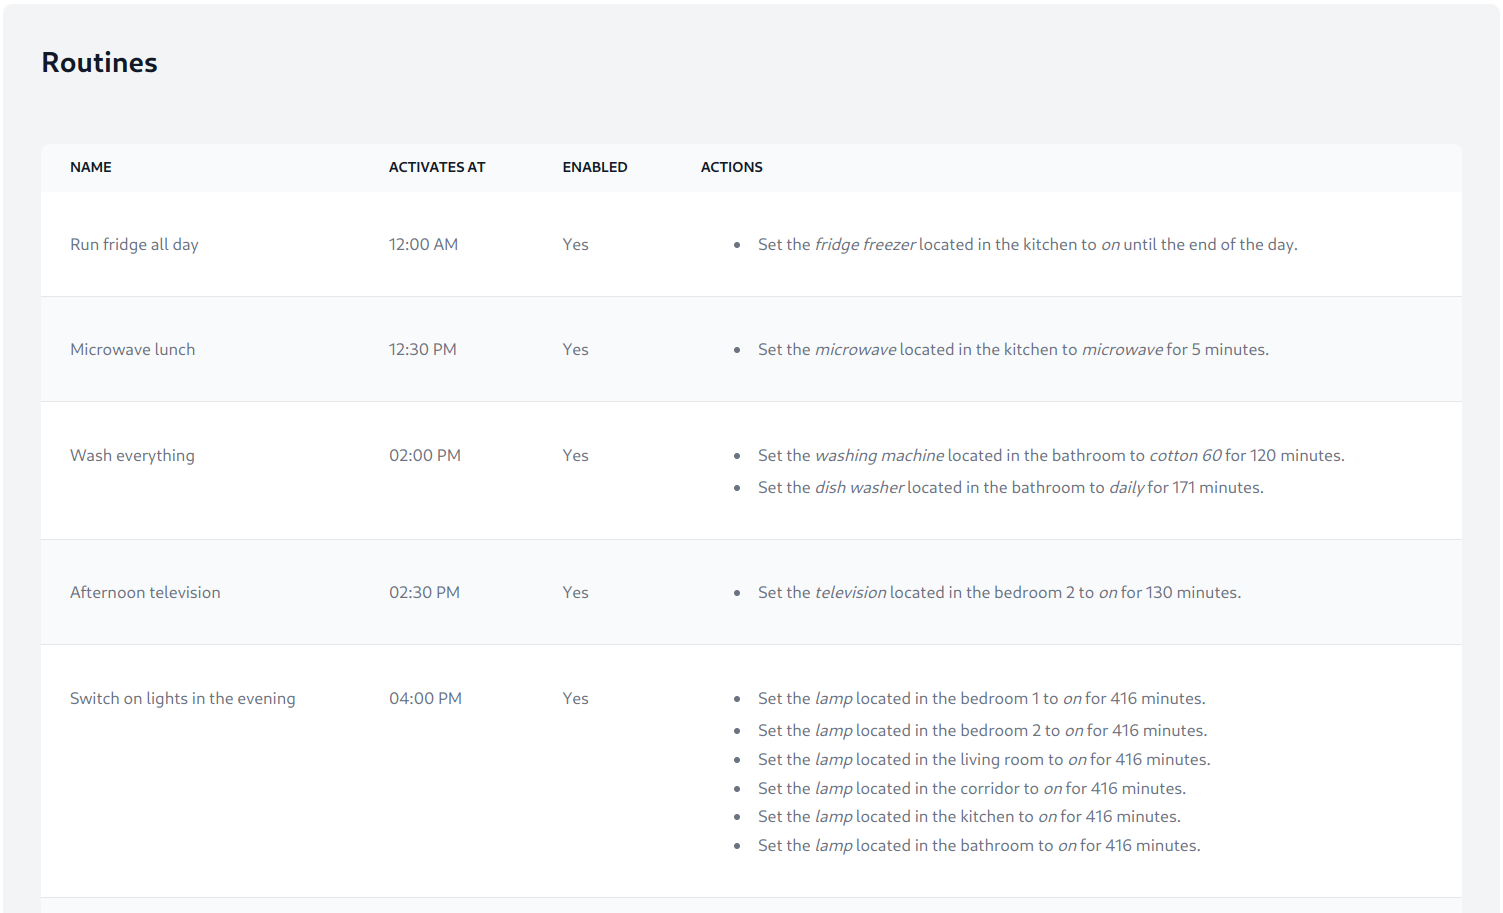
\includegraphics[width=0.9\textwidth]{images/frontend/routines.png}
    \caption{Showcase Frontend Application}
    \label{fig:frontend_routines}
\end{figure}